\documentclass{article}
\usepackage[brazil]{babel}
\usepackage[margin=1in]{geometry} 
\usepackage{amsmath,amsthm,amssymb,amsfonts, fancyhdr, color, comment, graphicx, environ}
\usepackage{xcolor}
\usepackage{mdframed}
\usepackage[shortlabels]{enumitem}
\usepackage{hyperref}
\usepackage{outlines}
\usepackage{amsmath}
\usepackage{listings}
\usepackage[utf8]{inputenc}
\usepackage{graphicx}


\usepackage{xcolor}

\definecolor{codegreen}{rgb}{0,0.6,0}
\definecolor{codegray}{rgb}{0.5,0.5,0.5}
\definecolor{codepurple}{rgb}{0.58,0,0.82}
\definecolor{backcolour}{rgb}{0.95,0.95,0.92}

\lstdefinestyle{estiloCod}{
    backgroundcolor=\color{backcolour},   
    commentstyle=\color{codegreen},
    keywordstyle=\color{magenta},
    numberstyle=\tiny\color{codegray},
    stringstyle=\color{codepurple},
    basicstyle=\ttfamily\footnotesize,
    breakatwhitespace=false,         
    breaklines=true,                 
    captionpos=b,                    
    keepspaces=true,                 
    numbers=left,                    
    numbersep=5pt,                  
    showspaces=false,                
    showstringspaces=false,
    showtabs=false,                  
    tabsize=2
}
\lstset{style=estiloCod}
\renewcommand{\lstlistingname}{Algoritmo}


\renewcommand{\footrulewidth}{0.8pt}
\hypersetup{
    colorlinks=true,
    linkcolor=blue,
    filecolor=magenta,      
    urlcolor=blue,
}

\pagestyle{fancy}

\newenvironment{problem}[2][Problem]
    { \begin{mdframed}[backgroundcolor=gray!20] \textbf{#1 #2} \\}
    {  \end{mdframed}}

\newenvironment{solution}{\textbf{Solution}}

\lhead{Lucas Elias de Andrade Cruvinel}
\rhead{Inteligência Artificial} 
\chead{\textbf{Trabalho 1}}
\lfoot{Sérgio Francisco}
\rfoot{Universidade Federal de Catalão}

\begin{document}
\title{\Large Inteligência Artificial \\[0.5cm]
        \bf\Large Trabalho 1: Resolução do Problema do Caixeiro Viajante por Simulated Annealing}
\author{\large Autor: Lucas Elias de Andrade Cruvinel\\ \ \\}

\makeatletter
    \begin{titlepage}
        \begin{center}
	   { 
\includegraphics[width=12cm]{UFCAT_-_Identidade_Visual_Original.png}}
	   {\ \\ \ \\}
        \vbox{}\vspace{5cm}
            {\@title }\\[3cm] 
            {\@author}
            {\large Professor: \bf Sérgio Francisco da Silva\\ \ \\}

        \end{center}
    \end{titlepage}
\makeatother
    \section{Problema do Caixeiro Viajante}
O Problema do Caixeiro Viajante (PCV), como nome sugere é baseado nos caixeiros que como trabalho tinham que ir de cidade à cidade para vender seus produtos de maneira nômade, e naturalmente um de seus problemas era a de saber qual seria o menor caminho a ser percorrido para chegar em determinada cidade.

De modo formal, transformando o conjunto de cidades em um grafo, pode ser dito que o problema do caixeiro viajante consiste na busca em um grafo do menor caminho possível de percorrer todos os nós conexos desse grafo.
    
Para solucionar o PCV, já foram desenvolvidos inúmeros algoritmos, dentre eles determinísticos ou de aproximação, em ambos os casos existem diversas que conseguem alcançar um resultado ótimo de maneira eficiente, porém mesmo assim continuam existindo sendo realizados estudos e pesquisas para encontrar evoluir tais algoritmos, isso acontece em parte por se tratar de um problema do conjunto NP-Completo e também por conta da utilização desse problema, tendo várias aplicabilidades em problemas da vida real dos mais variados tipos, como por exemplo processos industriais, mapeamento, combinação, entre outros.
    
    \section{Simulated Annealing}
O Simulated Annealing (SA) é um método de otimização é baseado no procedimento de recozimento usada na metalurgia em que um metal é esquentado para que possa ser esfriado lentamente para que os átomos possam se acalmar, desse modo retirando as imperfeições existentes. A principal característica desse método é que no começo o algoritmo tem uma grande probabilidade de aceitar ir para onde é classificado como ruim e conforme o tempo essa probabilidade vai diminuindo. Esse algoritmo pode então rodar até que essa probabilidade seja mínima ou depois de um número de iterações. O algoritmo é bem simples com uma teoria única porém pode ter diversos jeitos diferentes de ser executado.

\begin{outline}[enumerate]
    \1 Passo 1: Pegamos um ponto inicial via qualquer método, ex: Chute e também uma temperatura inicial.
    \1 Passo 2: Criar uma função que reduz a temperatura, geralmente se usa umas das 3 formas a seguir:
    \1 Passo 3: Usando a temperatura inicial, realizar n interações que realizam o passo 4, após cada uma dela realize a função que diminua a temperatura. As principais funções de redução de temperatura são:
    \2 Função de redução Linear
    \3 $T = T - \alpha$
    \2 Função de redução Geométrica
    \3 $T = T * \alpha$
    \2 Função de redução Lenta
    \3 $\dfrac{T}{(1 + \alpha T)}$
    \1 Passo 4: Esse passo será realizado em cada iteração: Pegue um ponto que seja vizinho do ponto atual, tire a função objetivo desse ponto, caso ela tenha um valor melhor(menor) ela será o novo ponto melhor e ponto atual, se não for, ela ainda tem chance usando cálculos de probabilidade, após esse cálculo se ela for aceita será o novo ponto atual, se novamente não for escolhida então é refeita com o ponto atual repetido.
  \end{outline}

A condição de parada pode ser acabar o número de iterações, a temperatura já estar muito baixa,  ou já ter achado um valor bom o suficiente.

O principal componente desse algoritmo é a temperatura que permite que pontos que não são bons ainda possam ser usados para sair de um mínimo local, porém se ele fosse verificar toda vez esses pontos ruins acabaria se tornando um algoritmo de força bruta por isso a temperatura inicial. Podemos dizer que no início o algoritmo está quente, com uma temperatura alta, o que faz ele tomar  mais ricos e verificar esses pontos ruins, porém, com o  tempo (com cada iteração), sua temperatura vai esfriando e então os esses pontos ruins começam a ser bem menos visitados para focar em achar o mínimo local.

\section{Ferramentas}
Para implementação deste trabalho foi utilizado a linguagem de programação Python 3, que é uma linguagem de fácil utilização no meio de manipulação de dados, por conta disso sendo de grande importância, além disso foram utilizadas algumas bibliotecas para auxílio principalmente na visualização de dados, sendo essas:

    \begin{itemize}
        \item Numpy, biblioteca de manipulação de listas e arrays que tem base em C, sendo muito mais rápido que a utilização nativa do Python.
        \item Matplotlib, biblioteca utilizada para representação gráfica do problema.
        \item Time, biblioteca de medição de tempo de execução do problema.
    \end{itemize}

\section{Parâmetros do Simulated Annealing}
Na inicialização do programa antes do início do algoritmo do Simulated Annealing são preparados variáveis que serão utilizadas para auxiliar o funcionamento da função ou para configurar. A principal configuração que molda todo o funcionamento da função são a temperatura inicial, temperatura mínima, valor e método de redução de temperatura, já que esses valores irão influenciar a probabilidade de aceitação de valores quando retornado o scores da função objetivo. Outras variáveis inicializadas são: número de cadeias de markov, que funcionam como número de iterações dentro de cada iteração do SA, criação de um score e um caminho inicial.

Nos casos de teste deste trabalho, o código é inicializado com:
\begin{itemize}
    \item Temperatura inicial: 100,0
    \item Temperatura mínima: 1,0
    \item Alfa: 0.98 (Sendo que a cada iteração T = T * alfa, resultando em uma redução geométrica)
    \item Número de cadeias de Markov: 100
\end{itemize}

O caminho inicial é feito através de um chute, de maneira aleatória, sendo o score inicial o cálculo deste. O que resta inicializar são os casos de teste, que são as cidades, estas também são criadas aleatoriamente, ao se gerar coordenadas aleatórias para representar tais, sendo guardadas em uma array numpy, de forma a ser um array de várias coordenadas, ficando com o formato (n, 2), sendo n o número de cidades.

\section{Formulação}
Como função objetivo deste problema é usado a distância total de se caminhar por todo o grafo, com isso em mente foi implementado a função \textit{calTourMileage}, nome derivado de ‘calcular a milhagem do Tour pela cidade’, que já expõe o objetivo de calcular a distância total ao se percorrer a cidade, que pode ser observada a seguir:

\begin{lstlisting}[language=Python, caption={Função Objetivo, cálculo distância do caminho.}]
# Calcula a distancia do caminho e serve como Funcao Objetivo
def calTourMileage(tourGiven, nCities, distMat):
    mileageTour = distMat[tourGiven[nCities-1], tourGiven[0]]   
    for i in range(nCities-1):                                  
        mileageTour += distMat[tourGiven[i], tourGiven[i+1]]
    return round(mileageTour)   # Arredonda o valor
\end{lstlisting}

A função recebe como parâmetros respectivamente o caminho a ser calculado, o número de cidades do problema, e uma matriz de adjacência com as distâncias. Com isso, a função consegue rodar um \textit{loop} que percorre todas as cidades e incrementando a variável auxiliar \textit{mileageTour} que salva a milhagem e depois é retornada.

Pega matriz de distâncias. Essa função recebe como parâmetros respectivamente o número de cidades e as coordenadas destas, e com isso monta uma matriz de duas dimensões para correlacionar as cidades, fazendo o cálculo de distância entre as cidades utilizando suas coordenadas. 

A função pode ser verificada a seguir:

\begin{lstlisting}[language=Python, caption={Função de criação de matriz de adjacência.}]
# Funcao para criar matriz de adjacencia entre as cidades com suas distancias
def getDistMat(nCities, coords):
    distMat = np.zeros((nCities,nCities))   # Inicializa uma matriz vazia
    for i in range(nCities):
        for j in range(i,nCities):
            distMat[i][j] = distMat[j][i] = round(np.linalg.norm(coords[i]-coords[j]))
    return distMat  
\end{lstlisting}

Outra função principal é a de realizar a perturbação na nossa amostra, nesse caso, no caminho, para isso é implementado a função \textit{MutateSwap} que realiza uma mudança e troca os caminhos, por exemplo em um conjunto de cidades {A, B e C}, onde A conecta com B, B conecta com C uma possível perturbação é mudar as conexões para que A conecte com C e C conecte com B. Dessa forma obtendo um novo caso que pode ser ou não melhor que o anterior, cabendo à função objetivo descobrir

A função recebe como parâmetros respectivamente o caminho a ser pertubado e a quantidade de cidades, em seu funcionamento, inicialmente é escolhido de forma aleatória uma cidade origem, e após isso uma cidade destino aleatória tomando cuidado para não ser a mesma que a de origem, após isso suas ligações são invertidas gerando e retornando um novo caminho.

Esta função pode ser verificada à seguir:

\begin{lstlisting}[language=Python, caption={Função de criação de matriz de adjacência.}]
# Pertuba o caminho atual trocando dois caminhos entre cidades
def mutateSwap(tourGiven, nCities):
    i = np.random.randint(nCities)          # Cria um valor aleatorio para cidade origem
    while True:
        j = np.random.randint(nCities)      # Cria um valor aleatorio para cidade destino
        if i!=j: break                      # Forcar destino diferente de origem 

    # Modifica o caminho dado e o retorna
    tourSwap = tourGiven.copy()       
    tourSwap[i],tourSwap[j] = tourGiven[j],tourGiven[i] # Inverte origem e destino
    return tourSwap
\end{lstlisting}

Para finalizar é implementado uma variável que salva o tempo atual antes do início do código para que possa ser comparada com o tempo depois da execução do código, fazendo com que se possa ter ideia do tempo consumido para execução do código, um exemplo desse método pode ser visto à seguir:

\begin{lstlisting}[language=Python, caption={Cálculo tempo de execução.}]
import time     # Biblioteca que implementa tais questoes
tempo_inicial = time.clock()    # Salva o tempo atual
#
#   Codigo a ser executado aqui
#
tempo_final = time.clock() - tempo_inicial  # Calculo do tempo de execucao
print(tempo_final)  # Exibe o resultado
\end{lstlisting}

\section{Desempenho}
Utilizando todos os parâmetros já discutidos, só resta verificar o resultado ao modificar o número de cidades.
Após os teste se encontrou os seguintes resultados:
\newpage
\begin{table}[h!]
    \begin{center}
      \caption{Casos de testes}
      \label{tab:table1}
      \begin{tabular}{|c||c|}
        \hline
        \textbf{Número de cidades} & \textbf{Tempo (segundos)}\\
        \hline
        10 & 0.020926237106323242\\\hline
        20 & 0.04984879493713379\\\hline
        50 & 0.19833922386169434\\\hline
        100 & 0.6538357734680176\\\hline
        250 & 3.747643232345581\\\hline
        500 & 15.012732744216919\\\hline
        1000 & 59.95423913002014\\\hline
        \hline
      \end{tabular}
    \end{center}
  \end{table}
  Como pode ser percebido o tempo gasto cresce de forma exponencial, justamente por isso esse problema não se enquadra nos problemas do tipo P, embora consiga ser redutível para NP-Completo, que é abaixo de exponencial.

  Pode ser de mais fácil a percepção de que é um problema exponencial utilizando a seguinte imagem:

  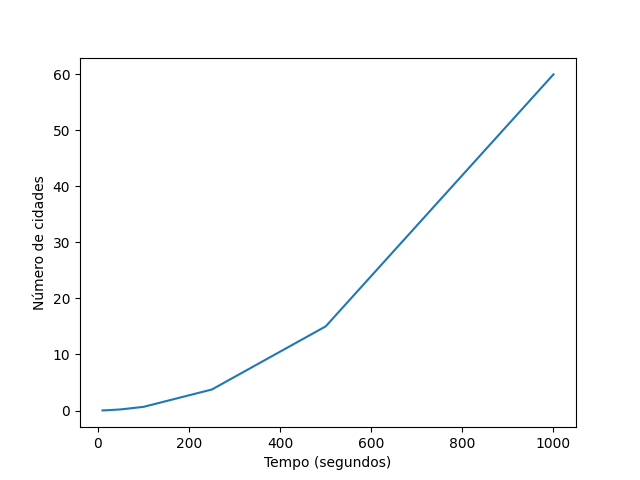
\includegraphics{fig1}

  \section{Conclusão}
  Embora possa ser percebido que com um grande número de cidades se torna ineficiente, para solucionar casos reais do problema do caixeiro viajante o simulated annealing é um bom algoritmo, já que nesses casos dificilmente se usarão casos que ultrapassem 100 cidades, contudo em algumas outras aplicações que utilizem o mesmo algoritmo, continua sendo uma boa alternativa em casos que não necessitem de milhares nós ou mais que isso.
  \section{Referências}

  \begin{enumerate}
    \item LAWLER, Eugène L.; RINNOOY-KAN, A. H. G.; LENSTRA, Jan Karel; SHMOYS, David B. – The Traveling salesman problem: a guided tour of combinatorial optimization. [S.l.]: Edição de Wiley, 1985. ISBN 978-0-471-90413-7
    \item REEVES, Colin R., ed. – Modern heuristic techniques for combinatorial problems. Ed. Colin R. Reeves. London: McGraw-Hill Book, 2000. XIII, 320 p..( Advanced Topic in Computer Science). ISBN 978-0-077-09239-9
    \item Franz, A.; Hoffmann, K.H.; Salamon, P (2001), "Best optimal strategy for finding ground states", Physical Review Letters, 86 (3): 5219–5222, doi:10.1103/PhysRevLett.86.5219, PMID 11384462
    \item Khachaturyan, A.; Semenovskaya, S.; Vainshtein, B. (1979). "Statistical-Thermodynamic Approach to Determination of Structure Amplitude Phases". Sov.Phys. Crystallography. 24 (5): 519–524.

\end{enumerate}
\end{document}